\documentclass[letter,10pt]{article}
\usepackage{latexsym}
\usepackage{amsmath}
\usepackage{amssymb}
\usepackage{amsthm}
\usepackage{amsfonts}
\usepackage{epsfig}
\usepackage{url}
\usepackage{fancyvrb}
\usepackage{hyperref}


%opening
\title{FLANN - Fast Library for Approximate Nearest Neighbors\\[0.5cm] User
Manual\\[1cm]}

\author{Marius Muja, mariusm@cs.ubc.ca\\David Lowe, lowe@cs.ubc.ca}


\begin{document}


 \begin{titlepage}
\vspace{10cm}
\maketitle
\thispagestyle{empty}
 \end{titlepage}


\section{Introduction}

We can define the \emph{nearest neighbor search (NSS)} problem in the
following way: given a set of points $P=p_1,p_2,\dots,p_n$ in a metric
space $X$, these points must be preprocessed in such a way that given a new
query point $q \in X$, finding the point in $P$ that is nearest to $q$ can
be done quickly.

The problem of nearest neighbor search is one of major importance in a
variety of applications such as image recognition, data compression,
pattern recognition and classification, machine learning,  document
retrieval systems, statistics and data analysis. However, solving this
problem in high dimensional spaces seems to be a very difficult task and
there is no algorithm that performs significantly better than the standard
brute-force search. This has lead to an increasing interest in a class of
algorithms that perform approximate nearest neighbor searches, which have
proven to be a good-enough approximation in most practical applications and
in most cases, orders of magnitude faster that the algorithms performing
the exact searches.

FLANN (Fast Library for Approximate Nearest Neighbors) is a library for
performing fast approximate nearest neighbor searches. FLANN is written in
the C++ programming language. FLANN can be easily used in many contexts
through the C, MATLAB and Python bindings provided with the library.



\subsection{Quick Start}
\label{sec:quickstart}


This section contains small examples of how to use the FLANN library from
different programming languages (C++, C, MATLAB and Python).

\begin{itemize}


\item \textbf{C++}
\begin{Verbatim}[fontsize=\scriptsize,frame=single]
// file flann_example.cpp

#include <flann/flann.hpp>
#include <flann/io/hdf5.h>

#include <stdio.h>

int main(int argc, char** argv)
{
    int nn = 3;

    flann::Matrix<float> dataset;
    flann::Matrix<float> query;
    flann::load_from_file(dataset, "dataset.hdf5","dataset");
    flann::load_from_file(query, "dataset.hdf5","query");

    flann::Matrix<int> indices(new int[query.rows*nn], query.rows, nn);
    flann::Matrix<float> dists(new float[query.rows*nn], query.rows, nn);

    // construct an randomized kd-tree index using 4 kd-trees
    flann::Index<flann::L2<float> > index(dataset, flann::KDTreeIndexParams(4));
    index.buildIndex();                                                                                               

    // do a knn search, using 128 checks
    index.knnSearch(query, indices, dists, nn, flann::SearchParams(128));

    flann::save_to_file(indices,"result.hdf5","result");

    delete[] dataset.ptr();
    delete[] query.ptr();
    delete[] indices.ptr();
    delete[] dists.ptr();
    
    return 0;
}

\end{Verbatim}


\item \textbf{C}
\begin{Verbatim}[fontsize=\scriptsize,frame=single]
/* file flann_example.c */

#include "flann.h"
#include <stdio.h>
#include <assert.h>

/* Function that reads a dataset */
float* read_points(char* filename, int *rows, int *cols);

int main(int argc, char** argv)
{
   int rows,cols;
   int t_rows, t_cols;
   float speedup;

   /* read dataset points from file dataset.dat */
   float* dataset = read_points("dataset.dat", &rows, &cols);
   float* testset = read_points("testset.dat", &t_rows, &t_cols);

   /* points in dataset and testset should have the same dimensionality */
   assert(cols==t_cols);

   /* number of nearest neighbors to search */
   int nn = 3;
   /* allocate memory for the nearest-neighbors indices */
   int* result = (int*) malloc(t_rows*nn*sizeof(int));                                                               
   /* allocate memory for the distances */
   float* dists = (float*) malloc(t_rows*nn*sizeof(float));

   /* index parameters are stored here */
   struct FLANNParameters p = DEFAULT_FLANN_PARAMETERS;
   p.algorithm = FLANN_INDEX_AUTOTUNED;  /* or FLANN_INDEX_KDTREE, FLANN_INDEX_KMEANS, ... /*
   p.target_precision = 0.9;  /* want 90% target precision */

   /* compute the 3 nearest-neighbors of each point in the testset */
   flann_find_nearest_neighbors(dataset, rows, cols, testset, t_rows,
result, dists, nn, &p);

   ...
   free(dataset);
   free(testset);
   free(result);
   free(dists);

   return 0;
}

\end{Verbatim}



\item \textbf{MATLAB}
\begin{Verbatim}[fontsize=\scriptsize,frame=single]
% create random dataset and test set
dataset = single(rand(128,10000));
testset = single(rand(128,1000));

% define index and search parameters
params.algorithm = 'kdtree';
params.trees = 8;
params.checks = 64;

% perform the nearest-neighbor search
[result, dists] = flann_search(dataset,testset,5,params);
\end{Verbatim}

\item \textbf{Python}
\begin{Verbatim}[fontsize=\scriptsize,frame=single]
from pyflann import *
from numpy import *
from numpy.random import *

dataset = rand(10000, 128)
testset = rand(1000, 128)

flann = FLANN()
result,dists = flann.nn(dataset,testset,5,algorithm="kmeans",
               branching=32, iterations=7, checks=16);
\end{Verbatim}

\end{itemize}



\section{Downloading and compiling FLANN}
\label{sec:downloading_and_compiling}

FLANN can be downloaded from the following address:
\begin{center}
\texttt{http://www.cs.ubc.ca/$\sim$mariusm/flann}
\end{center}

After downloading and unpacking, the following files and directories should
be present:
\begin{itemize}
\item \texttt{bin}: directory various for scripts and binary files
\item \texttt{doc}: directory containg this documentation
\item \texttt{examples}: directory containg examples of using FLANN
\item \texttt{src}: directory containg the source files
\item \texttt{test}: directory containg unit tests for FLANN
\end{itemize}



To compile the FLANN library the \textit{CMake}\footnote{http://www.cmake.org/} build system is required.
Below is an example of how FLANN can be compiled on Linux (replace x.y.z with the corresponding version number).
\begin{Verbatim}[fontsize=\scriptsize,frame=single]
$ cd flann-x.y.z-src
$ mkdir build
$ cd build
$ cmake ..
$ make
\end{Verbatim}

On windows the steps are very similar:
 
\begin{Verbatim}[fontsize=\scriptsize,frame=single]
> "C:\Program Files\Microsoft Visual Studio 9.0\VC\vcvarsall.bat"
> cd flann-x.y.z-src
> mkdir build
> cd build
> cmake ..
> nmake
\end{Verbatim}

There are several compile options that can be configured before FLANN is compiled, for example the build type 
(Release, RelWithDebInfo, Debug) or whether to compile the C, Python or the MATLAB bindings. To change any of this
options use the \texttt{cmake-gui} application after \texttt{cmake} has finished (see figure \ref{fig:cmake-gui}).
\begin{Verbatim}[fontsize=\scriptsize,frame=single]
> cmake-gui .
\end{Verbatim}

\begin{figure}[h]
  \begin{center}
    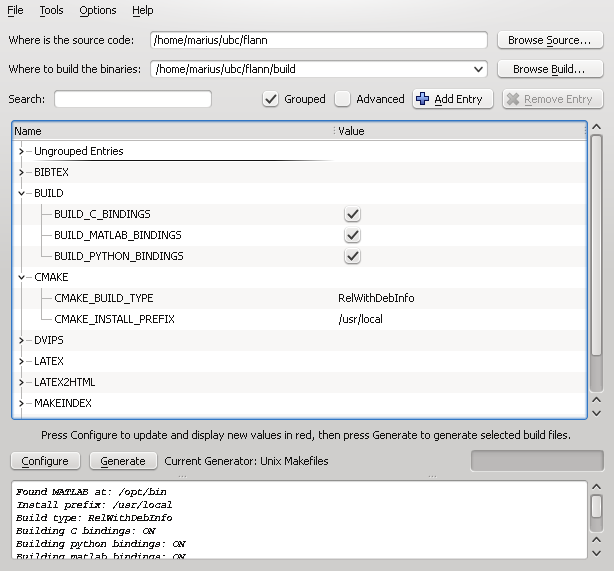
\includegraphics[width=0.9\textwidth]{images/cmake-gui.png}
    \caption{Configuring the FLANN compile options}
    \label{fig:cmake-gui}
  \end{center}
\end{figure}

\subsection{Upgrading from a previous version}

This section contains changes that you need to be aware of when upgrading from a previous version of FLANN.

\begin{description}
 \item[Version 1.7.0] A small breaking API change in \texttt{flann::Matrix} requires client code to be updated. In order
to release the memory used by a matrix, use:
\begin{Verbatim}[fontsize=\scriptsize]
 delete[] matrix.ptr();
\end{Verbatim}
instead of:
\begin{Verbatim}[fontsize=\scriptsize]
 delete[] matrix.data;
\end{Verbatim}
or:
\begin{Verbatim}[fontsize=\scriptsize]
 matrix.free();
\end{Verbatim}
The member \texttt{data} of \texttt{flann::Matrix} is not publicly accessible any more, use the \texttt{ptr()} method
to obtain the pointer to the memory buffer.
\end{description}



\subsection{Compiling FLANN with multithreading support}

For taking advantage of multithreaded search, the project that uses FLANN needs to be compiled with a compiler that 
supports the OpenMP standard and the OpenMP support must be enabled. The number of cores to be used can be selected with 
the \texttt{cores} field in the \texttt{SearchParams} structure. By default a single core will be used. 
Setting the \texttt{cores} field to zero will automatically use as many threads as cores available on the machine.

\section{Using FLANN}

\subsection{Using FLANN from C++}

The core of the FLANN library is written in C++. To make use of the full power 
and flexibility of the templated code one should use the C++ bindings if possible. 
To use the C++ bindings you only need to include the  the library header file \texttt{flann.hpp}. An example
of the compile command that must be used will look something like this:
\begin{Verbatim}[fontsize=\footnotesize]
g++ flann_example.cpp -I $FLANN_ROOT/include -o flann_example_cpp
\end{Verbatim}
where \texttt{\$FLANN\_ROOT} is the library main directory.

The following sections describe the public C++ API.

\subsubsection{flann::Index}
\label{sec:flann::Index}
The FLANN nearest neighbor index class. This class is used to abstract different types of nearest neighbor search
indexes. The class is templated on the distance functor to be used for computing distances between pairs of features. 

\begin{Verbatim}[fontsize=\footnotesize,frame=single]
namespace flann
{
    template<typename Distance>
    class Index 
    {
	typedef typename Distance::ElementType ElementType;
	typedef typename Distance::ResultType DistanceType;
    public:
        Index(const IndexParams& params, Distance distance = Distance() );
        
        Index(const Matrix<ElementType>& points, const IndexParams& params,
                Distance distance = Distance() );

	~Index();

	void buildIndex();        
        
        void buildIndex(const Matrix<ElementType>& points);
        
        void addPoints(const Matrix<ElementType>& points, 
                       float rebuild_threshold = 2);
        
        void removePoint(size_t point_id);
        
        ElementType* getPoint(size_t point_id);

	int knnSearch(const Matrix<ElementType>& queries, 
		       Matrix<int>& indices, 
		       Matrix<DistanceType>& dists, 
		       size_t knn, 
		       const SearchParams& params);

        int knnSearch(const Matrix<ElementType>& queries,
                       std::vector< std::vector<int> >& indices,
                       std::vector<std::vector<DistanceType> >& dists,
                       size_t knn,
                       const SearchParams& params);

	int radiusSearch(const Matrix<ElementType>& queries, 
			 Matrix<int>& indices, 
			 Matrix<DistanceType>& dists, 
			 float radius, 
			 const SearchParams& params);

        int radiusSearch(const Matrix<ElementType>& queries,
                          std::vector< std::vector<int> >& indices,
                          std::vector<std::vector<DistanceType> >& dists,
                          float radius,
                          const SearchParams& params);

	void save(std::string filename);

	int veclen() const;

	int size() const;

	IndexParams getParameters() const;

        flann_algorithm_t getType() const;

    };
}
\end{Verbatim}


\textbf{The Distance functor}

The distance functor is a class whose \texttt{operator()} computes the distance between two features. If the distance is
also a kd-tree compatible distance it should also provide an \texttt{accum\_dist()} method that computes the distance
between individual feature dimensions. A typical distance functor looks like this (see the \texttt{dist.h} file for more
examples):

\begin{Verbatim}[fontsize=\footnotesize,frame=single]
template<class T>
struct L2
{
    typedef bool is_kdtree_distance;

    typedef T ElementType;
    typedef typename Accumulator<T>::Type ResultType;

    template <typename Iterator1, typename Iterator2>
    ResultType operator()(Iterator1 a, Iterator2 b, size_t size, 
                          ResultType /*worst_dist*/ = -1) const
    {
        ResultType result = ResultType();
        ResultType diff;
        for(size_t i = 0; i < size; ++i ) {
            diff = *a++ - *b++;
            result += diff*diff;
        }
        return result;
    }

    template <typename U, typename V>
    inline ResultType accum_dist(const U& a, const V& b, int) const
    {
        return (a-b)*(a-b);
    }
};
\end{Verbatim}

In addition to \texttt{operator()} and \texttt{accum\_dist()}, a distance functor should also define the
\texttt{ElementType} and the \texttt{ResultType} as the types of the elements it operates on and the type of the result
it computes.

If a distance functor can be used as a kd-tree distance (meaning that the full distance between a pair of features can
be accumulated from the partial distances between the individual dimensions) a typedef \texttt{is\_kdtree\_distance}
should be present inside the distance functor. If the distance is not a kd-tree distance, but it's a distance in a
vector space (the individual dimensions of the elements it operates on can be accessed independently) a typedef
\texttt{is\_vector\_space\_distance} should be defined inside the functor. If neither typedef is defined, the distance
is assumed to be a metric distance and will only be used with indexes operating on generic metric distances.
\\


\textbf{flann::Index::Index}
Constructs a nearest neighbor search index for a given dataset.
\begin{Verbatim}[fontsize=\footnotesize,frame=single]
Index(const IndexParams& params, Distance distance = Distance() );

Index(const Matrix<ElementType>& points, const IndexParams& params,
        Distance distance = Distance() );
\end{Verbatim}
\begin{description}
\item[features] Matrix containing the features(points) that should be indexed, stored in a row-major order (one point 
on each row of the matrix). The size of the matrix is $num\_features \times dimensionality$.

\item[params] Structure containing the index parameters. The type of index that will be constructed depends on the type 
of this parameter. The possible parameter types are:

\textbf{LinearIndexParams} When passing an object of this type, the index will perform a linear, brute-force search.
\begin{Verbatim}[fontsize=\footnotesize]
struct LinearIndexParams : public IndexParams 
{
};
\end{Verbatim}

\textbf{KDTreeIndexParams} When passing an object of this type the index constructed will consist of a set 
of randomized kd-trees which will be searched in parallel.
\begin{Verbatim}[fontsize=\footnotesize]
struct KDTreeIndexParams : public IndexParams
{
      KDTreeIndexParams( int trees = 4 );
};
\end{Verbatim}
\begin{description}
 \item[trees] The number of parallel kd-trees to use. Good values are in the range [1..16]
\end{description}

\textbf{KMeansIndexParams} When passing an object of this type the index constructed will be a hierarchical k-means tree. 
\begin{Verbatim}[fontsize=\footnotesize]
struct KMeansIndexParams : public IndexParams
{
	KMeansIndexParams( int branching = 32,
			int iterations = 11,
			flann_centers_init_t centers_init = FLANN_CENTERS_RANDOM,
			float cb_index = 0.2 );
};
\end{Verbatim}
\begin{description}
\item[branching]{ The branching factor to use for the hierarchical k-means tree }
\item[iterations]{ The maximum number of iterations to use in the k-means clustering 
		    stage when building the k-means tree. If a value of -1 is used here, it means
		    that the k-means clustering should be iterated until convergence}
\item[centers\_init]{ The algorithm to use for selecting the initial
		  centers when performing a k-means clustering step. The possible values are
		  CENTERS\_RANDOM (picks the initial cluster centers randomly), CENTERS\_GONZALES (picks the
		  initial centers using Gonzales' algorithm) and CENTERS\_KMEANSPP (picks the initial
		centers using the algorithm suggested in \cite{arthur_kmeanspp_2007}) }
\item[cb\_index]{ This parameter (cluster boundary index) influences the
		  way exploration is performed in the hierarchical kmeans tree. When \texttt{cb\_index} is zero
		  the next kmeans domain to be explored is choosen to be the one with the closest center. 
		  A value greater then zero also takes into account the size of the domain.}
\end{description}


\textbf{CompositeIndexParams} When using a parameters object of this type the index created combines the randomized
kd-trees 
        and the hierarchical k-means tree.
\begin{Verbatim}[fontsize=\footnotesize]
struct CompositeIndexParams : public IndexParams
{
        CompositeIndexParams( int trees = 4,
                          int branching = 32,
                          int iterations = 11,
                          flann_centers_init_t centers_init = FLANN_CENTERS_RANDOM, 
                          float cb_index = 0.2 );
};
\end{Verbatim}


\textbf{KDTreeSingleIndexParams} When passing an object of this type the index will contain a single kd-tree
optimized for searching lower dimensionality data (for example 3D point clouds)
\begin{Verbatim}[fontsize=\footnotesize]
struct KDTreeSingleIndexParams : public IndexParams
{
      KDTreeSingleIndexParams( int leaf_max_size = 10 );
};
\end{Verbatim}
\begin{description}
 \item[max\_leaf\_size] The maximum number of points to have in a leaf for not branching the tree any more.
\end{description}

\textbf{KDTreeCuda3dIndexParams} When passing an object of this type the index will be a single kd-tree that 
is built and performs searches on a CUDA compatible GPU. Search performance is best for large numbers of search and query points.
For more information, see section \ref{sec:flann::cuda}
\begin{Verbatim}[fontsize=\footnotesize]
struct KDTreeCuda3dIndexParams : public IndexParams
{
    KDTreeCuda3dIndexParams( int leaf_max_size = 64 );
};
\end{Verbatim}
\begin{description}
 \item[max\_leaf\_size] The maximum number of points to have in a leaf for not branching the tree any more.
\end{description}


\textbf{HierarchicalClusteringIndexParams} When passing an object of this type the index constructed will be a
hierarchical clustering index. This type of index works with any metric distance and can be used for matching 
binary features using Hamming distances.
\begin{Verbatim}[fontsize=\footnotesize]
struct HierarchicalClusteringIndexParams : public IndexParams
{
    HierarchicalClusteringIndexParams(int branching = 32,
                              flann_centers_init_t centers_init = FLANN_CENTERS_RANDOM,
                              int trees = 4, int leaf_max_size = 100)
};
\end{Verbatim}
\begin{description}
\item[branching]{ The branching factor to use for the hierarchical clustering tree }
\item[centers\_init]{ The algorithm to use for selecting the initial
                  centers when performing a k-means clustering step. The possible values are
                  CENTERS\_RANDOM (picks the initial cluster centers randomly), CENTERS\_GONZALES (picks the
                  initial centers using Gonzales' algorithm) and CENTERS\_KMEANSPP (picks the initial
                centers using the algorithm suggested in \cite{arthur_kmeanspp_2007}) }
\item[trees] The number of parallel trees to use. Good values are in the range [3..8]
\item[leaf\_size] The maximum number of points a leaf node should contain.
\end{description}


\textbf{LshIndexParams} When passing an object of this type the index constructed will be a multi-probe LSH
(Locality-Sensitive Hashing) index. This type of index can only be used for matching binary features using Hamming
distances.
\begin{Verbatim}[fontsize=\footnotesize]
struct LshIndexParams : public IndexParams
{
    LshIndexParams(unsigned int table_number = 12, 
                  unsigned int key_size = 20, 
                  unsigned int multi_probe_level = 2);
};
\end{Verbatim}
\begin{description}
\item[table\_number]{ The number of hash tables to use }
\item[key\_size]{ The length of the key in the hash tables}
\item[multi\_probe\_level] Number of levels to use in multi-probe (0 for standard LSH)
\end{description}


\textbf{AutotunedIndexParams}
  When passing an object of this type the index created is automatically tuned to offer 
the best performance, by choosing the optimal index type (randomized kd-trees, hierarchical kmeans, linear) and parameters for the
dataset provided.
\begin{Verbatim}[fontsize=\footnotesize]
struct AutotunedIndexParams : public IndexParams
{
	AutotunedIndexParams( float target_precision = 0.9,
			  float build_weight = 0.01,
			  float memory_weight = 0,
			  float sample_fraction = 0.1 );
};
\end{Verbatim}
\begin{description}
\item[target\_precision]{ Is a number between 0 and 1 specifying the
percentage of the approximate nearest-neighbor searches that return the
exact nearest-neighbor. Using a higher value for this parameter gives
more accurate results, but the search takes longer. The optimum value
usually depends on the application. }

\item[build\_weight]{ Specifies the importance of the
index build time raported to the nearest-neighbor search time. In some
applications it's acceptable for the index build step to take a long time
if the subsequent searches in the index can be performed very fast. In
other applications it's required that the index be build as fast as
possible even if that leads to slightly longer search times.}

\item[memory\_weight]{Is used to specify the tradeoff between
time (index build time and search time) and memory used by the index. A
value less than 1 gives more importance to the time spent and a value
greater than 1 gives more importance to the memory usage.}

\item[sample\_fraction]{Is a number between 0 and 1 indicating what fraction
of the dataset to use in the automatic parameter configuration algorithm. Running the 
algorithm on the full dataset gives the most accurate results, but for
very large datasets can take longer than desired. In such case using just a fraction of the
data helps speeding up this algorithm while still giving good approximations of the
optimum parameters.}
\end{description}

\textbf{SavedIndexParams}
This object type is used for loading a previously saved index from the disk.
\begin{Verbatim}[fontsize=\footnotesize]
struct SavedIndexParams : public IndexParams
{
      SavedIndexParams( std::string filename );
};
\end{Verbatim}
\begin{description}
\item[filename]{ The filename in which the index was saved. }
\end{description}
\end{description}

\subsubsection{flann::Index::buildIndex}
Builds the nearest neighbor search index. There are two versions of the \texttt{buildIndex} method, one that
uses the points provided as argument and one that uses the points provided to the constructor when the object was
constructed.
\begin{Verbatim}[fontsize=\footnotesize,frame=single]
void buildIndex();        

void buildIndex(const Matrix<ElementType>& points);
\end{Verbatim}

\subsubsection{flann::Index::addPoints}
The \texttt{addPoints} method can be used to incrementally add points to the index after the index was build.
To avoid the index getting unbalanced, the \texttt{addPoints} method has the option of rebuilding the index after a
large number of points have been added. The \texttt{rebuild\_threshold} parameter controls when the index is
rebuild, by default this is done when it doubles in size (\texttt{rebuild\_threshold} = 2).

\begin{Verbatim}[fontsize=\footnotesize,frame=single]
void addPoints(const Matrix<ElementType>& points, float rebuild_threshold = 2);
\end{Verbatim}

\subsubsection{flann::Index::removePoint}
The \texttt{removePoint} method removes one point with the specified \texttt{point\_id} from the index. The indices
 (of the remaining points) returned by the nearest neighbor operations do not change when points are removed from the
index.

\begin{Verbatim}[fontsize=\footnotesize,frame=single]
void removePoint(size_t point_id);
\end{Verbatim}

\subsubsection{flann::Index::getPoint}
The \texttt{getPoint} method returns a pointer to the data point with the specified \texttt{point\_id}.

\begin{Verbatim}[fontsize=\footnotesize,frame=single]
ElementType* getPoint(size_t point_id);
\end{Verbatim}

\subsubsection{flann::Index::knnSearch}
Performs a K-nearest neighbor search for a set of query points. There are two signatures for this
method, one that takes pre-allocated \texttt{flann::Matrix} objects for returning the indices of and distances to the
neighbors found, and one that takes \texttt{std::vector<std::vector>} that will re resized automatically as needed.
\begin{Verbatim}[fontsize=\footnotesize,frame=single]
int Index::knnSearch(const Matrix<ElementType>& queries,
		Matrix<int>& indices, 
		Matrix<DistanceType>& dists,
		size_t knn,
		const SearchParams& params);

int Index::knnSearch(const Matrix<ElementType>& queries,
                std::vector< std::vector<int> >& indices,
                std::vector<std::vector<DistanceType> >& dists,
                size_t knn,
                const SearchParams& params);
\end{Verbatim}
\begin{description}
\item[queries]{Matrix containing the query points. Size of matrix is ($num\_queries \times dimentionality $)}
\item[indices]{Matrix that will contain the indices of the K-nearest neighbors found (size should be at least
$num\_queries \times knn$ for the pre-allocated version).}
\item[dists]{Matrix that will contain the distances to the K-nearest neighbors found (size should be at least
$num\_queries \times knn$ for the pre-allocated version).}
\item[knn]{Number of nearest neighbors to search for.}
\item[params]{Search parameters.} Structure containing parameters used during search.

\textbf{SearchParameters}
\begin{Verbatim}[fontsize=\footnotesize]
struct SearchParams
{
	SearchParams(int checks = 32,
		  float eps = 0,
		  bool sorted = true);

    int checks;
    float eps;
    bool sorted;
    int max_neighbors;
    tri_type use_heap;
    int cores;
    bool matrices_in_gpu_ram;
};
\end{Verbatim}
\begin{description}
 \item[checks] specifies the maximum leafs to visit when searching for neighbours. A
higher value for this parameter would give better search precision, but
also take more time. For all leafs to be checked use the value \texttt{CHECKS\_UNLIMITED}.
If automatic configuration was used when the index was created, the number of checks 
required to achieve the specified precision was also computed, to use that value specify \texttt{CHECKS\_AUTOTUNED}.
 \item[eps] Search for eps-approximate neighbors (only used by KDTreeSingleIndex and KDTreeCuda3dIndex).
 \item[sorted] Used only by radius search, specifies if the neighbors returned should be sorted by distance.
 \item[max\_neighbours] Specifies the maximum number of neighbors radius search should return (default: -1 =
unlimited). Only used for radius search.
 \item[use\_heap] Use a heap data structure to manage the list of neighbors internally (possible values: FLANN\_False,
FLANN\_True, FLANN\_Undefined). A heap is more efficient for a large number of neighbors and less efficient for a small
number of neighbors. Default value is FLANN\_Undefined, which lets the code choose the best option depending on the
number of neighbors requested. Only used for KNN search.
 \item[cores] How many cores to assign to the search (specify 0 for automatic core selection).
 \item[matrices\_in\_gpu\_ram] for GPU search indicates if matrices are already in GPU ram.
\end{description}
\end{description}


\subsubsection{flann::Index::radiusSearch}
Performs a radius nearest neighbor search for a set of query points. There are two signatures for this method,
one that takes pre-allocated \texttt{flann::Matrix} objects for returning the indices of and distances to the neighbors
found, and one that takes \texttt{std::vector<std::vector>} that will resized automatically as needed.
\begin{Verbatim}[fontsize=\footnotesize,frame=single]
int Index::radiusSearch(const Matrix<ElementType>& queries,
		  Matrix<int>& indices,
		  Matrix<DistanceType>& dists,
		  float radius,
		  const SearchParams& params); 

int Index::radiusSearch(const Matrix<ElementType>& queries,
                  std::vector< std::vector<int> >& indices,
                  std::vector<std::vector<DistanceType> >& dists,
                  float radius,
                  const SearchParams& params);
\end{Verbatim}

\begin{description}
\item[queries]{The query point. Size of matrix is ($num\_queries \times dimentionality $).}
\item[indices]{Matrix that will contain the indices of the K-nearest neighbors found. For the pre-allocated version,
only as many neighbors are returned as many columns in this matrix. If fewer neighbors are found than
columns in this matrix, the element after that last index returned is -1. In case of the std::vector version, the rows
will be resized as needed to fit all the neighbors to be returned, except if the ``max\_neighbors'' search parameter is
set.}
\item[dists]{Matrix that will contain the distances to the K-nearest neighbors found. The same number of values are
returned here as for the \texttt{indices} matrix.}
\item[radius]{The search radius}
\item[params]{Search parameters}
\end{description}
The method returns the number of nearest neighbors found.


\subsubsection{flann::Index::save}
Saves the index to a file.
\begin{Verbatim}[fontsize=\footnotesize,frame=single]
  void Index::save(std::string filename);
\end{Verbatim}
\begin{description}
\item[filename]{The file to save the index to}
\end{description}

\subsubsection{flann::hierarchicalClustering}
\label{flann::hierarchicalClustering}
Clusters the given points by constructing a hierarchical k-means tree and choosing a cut in the tree that minimizes the clusters' variance.

\begin{Verbatim}[fontsize=\footnotesize,frame=single]
template <typename Distance>
int hierarchicalClustering(const Matrix<typename Distance::ElementType>& features, 
			Matrix<typename Distance::ResultType>& centers,
			const KMeansIndexParams& params, 
		        Distance d = Distance())
\end{Verbatim}
\begin{description}
\item[features]{The points to be clustered}
\item[centers]{The centers of the clusters obtained. The number of rows in this matrix represents the number of clusters desired.
However, because of the way the cut in the hierarchical tree is choosen, the number of clusters computed will be
 the highest number of the form $(branching-1)*k+1$ that's lower than the number of clusters desired, where $branching$ is the tree's 
branching factor (see description of the KMeansIndexParams).  }
\item[params]{Parameters used in the construction of the hierarchical k-means tree}
\end{description}
The function returns the number of clusters computed.

\subsubsection{flann::KdTreeCuda3dIndex}
\label{sec:flann::cuda}
FLANN provides a CUDA implementation of the kd-tree build and search algorithms to improve the build and query speed for large 3d data sets. This section will provide all the necessary information to use the \texttt{KdTreeCuda3dIndex} index type.

\textbf{Building:}
If CMake detects a CUDA install during the build (see section \ref{sec:downloading_and_compiling}), a library \texttt{libflann\_cuda.so} will be built. 

\textbf{Basic Usage:}
To be able to use the new index type, you have to include the FLANN header this way:
\begin{Verbatim}[fontsize=\footnotesize,frame=single]
#define FLANN_USE_CUDA
#include <flann/flann.hpp>
\end{Verbatim}
If you define the symbol \texttt{FLANN\_USE\_CUDA} before including the FLANN header, you will have to link \texttt{libflann\_cuda.so} or \texttt{libflann\_cuda\_s.a} with your project. 
However, you will not have to compile your source code with \texttt{nvcc}, except if you use other CUDA code, of course.

You can then create your index by using the \texttt{KDTreeCuda3dIndexParams} to create the index. The index will take care of copying all the data from and to the GPU for you, both 
for index creation and search.

A word of caution: A general guideline for deciding whether to use the CUDA kd tree or a (multi-threaded) CPU implementation is hard to give, since it depends on the combination of CPU and GPU in each system and the data sets.
For example, on a system with a Phenom II 955 CPU and a Geforce GTX 260 GPU, the maximum search speedup on a synthetic (random) data set is a factor of about 8-9 vs the single-core CPU search, and starts to be reached at about 100k search and query points. (This includes transfer times.)
Build time does not profit as much from the GPU acceleration; here the benefit is about 2x at 200k points, but this largely depends on the data set. The only way to know which implementation is best suited is to try it.

\textbf{Advanced Usage:}
In some cases, you might already have your data in a buffer on the GPU. In this case, you can re-use these buffers instead of copying the buffers back to system RAM for index creation and search.
The way to do this is to pass GPU pointers via the \texttt{flann::Matrix} inputs and tell the index via the index and search params to treat the pointers as GPU pointers.
\begin{Verbatim}[fontsize=\footnotesize,frame=single]
thrust::device_vector<float4>  points_vector( n_points );
// ... fill vector here...

float* gpu_pointer = (float*)thrust::raw_pointer_cast(&points_vector[0]);
flann::Matrix<float> matrix_gpu(gpu_pointer,n_points,3, 4);

flann::KDTreeCuda3dIndexParams params;
params["input_is_gpu_float4"]=true;
flann::Index<flann::L2<float> > flannindex( matrix_gpu, params  );
flannindex.buildIndex();
\end{Verbatim}
\begin{description}
 \item First, a GPU buffer of float4 values is created and filled with points. \footnote{For index creation, only \texttt{float4} points are supported, \texttt{float3} or structure-of-array (SOA) representations are currently not supported since
\texttt{float4} proved to be best in terms of access speed for tree creation and search.}
 \item Then, a GPU pointer to the buffer is stored in a flann matrix with 3 columns and a stride of 4 (since the last element in the \texttt{float4} is unused).
 \item Last, the index is created. The \texttt{input\_is\_gpu\_float4} flag tells the index to treat the matrix as a gpu buffer.
\end{description}

Similarly, you can specify GPU buffers for the search routines that return the result via flann matrices (but not for those that return them via \texttt{std::vector}s).
To do this, the pointers in the index and dist matrices have to point to GPU buffers and the \texttt{cols} value has to be set to 3 (as we are dealing with 3d points). Here, any value for \texttt{stride} can be used.
\begin{Verbatim}[fontsize=\footnotesize,frame=single]
flann::Matrix<int> indices_gpu(gpu_pointer_indices,n_points, knn, stride);
flann::Matrix<float> dists_gpu(gpu_pointer_dists,n_points, knn, stride);

flann::SearchParams params;
params.matrices_in_gpu_ram = true;

flannindex.knnSearch( queries_gpu ,indices_gpu,dists_gpu,knn, params);
\end{Verbatim}
\begin{description}
 \item Note that you cannot mix matrices in system and CPU ram here!
\end{description}

\textbf{Search Parameters:}
The search routines support three parameters:
\begin{itemize}
 \item \texttt{eps} - used for approximate knn search. The maximum possible error is $e= d_{best} * eps$, i.e. the distance of the returned neighbor is at maximum $eps$ times larget than the distance to the real best neighbor.
 \item \texttt{use\_heap} - used in knn and radius search. If set to true, a heap structure will be used in the search to keep track of the distance to the farthest neighbor. Beneficial with about $k>64$ elements.
 \item \texttt{sorted} - if set to true, the results of the radius and knn searches will be sorted in ascending order by their distance to the query point.
 \item \texttt{matrices\_in\_gpu\_ram} - set to true to indicate that all (input and output) matrices are located in GPU RAM.
\end{itemize}


\subsection{Using FLANN from C}

FLANN can be used in C programs through the C bindings provided
with the library. Because there is no template support in C, there
are bindings provided for the following data types: \texttt{unsigned char},
\texttt{int}, \texttt{float} and \texttt{double}. For each of the functions 
below there is a corresponding version for each of the for data types, for example
for the function:
\begin{Verbatim}[fontsize=\footnotesize,frame=single]
flan_index_t flann_build_index(float* dataset, int rows, int cols, float* speedup,
	struct FLANNParameters* flann_params);
\end{Verbatim}
there are also the following versions:
\begin{Verbatim}[fontsize=\footnotesize,frame=single]
flan_index_t flann_build_index_byte(unsigned char* dataset,
	int rows, int cols, float* speedup,
	struct FLANNParameters* flann_params);
flan_index_t flann_build_index_int(int* dataset,
	int rows, int cols, float* speedup,
	struct FLANNParameters* flann_params);
flan_index_t flann_build_index_float(float* dataset,
	int rows, int cols, float* speedup,
	struct FLANNParameters* flann_params);
flan_index_t flann_build_index_double(double* dataset,
	int rows, int cols, float* speedup,
	struct FLANNParameters* flann_params);
\end{Verbatim}

\subsubsection{flann\_build\_index()}
\begin{Verbatim}[fontsize=\footnotesize,frame=single]
flan_index_t flann_build_index(float* dataset,
	int rows,
	int cols,
	float* speedup,
	struct FLANNParameters* flann_params);
\end{Verbatim}
This function builds an index and return a reference to it. The arguments
expected by this function are as follows:
\begin{description}
 \item[dataset, rows and cols] - are used to specify the input dataset of
points: dataset is a pointer to a $\rm{rows} \times \rm{cols}$ matrix
stored in row-major order (one feature on each row)
\item [speedup] - is used to return the approximate speedup over linear
search achieved when using the automatic index and parameter configuration
(see section \ref{sec:flann_build_index})
\item [flann\_params] - is a structure containing the parameters passed to
the function. This structure is defined as follows:
\begin{Verbatim}[fontsize=\footnotesize]
struct FLANNParameters {
  enum flann_algorithm_t algorithm; 	/* the algorithm to use */

  /* search parameters */
  int checks;            /* how many leafs (features) to check in one search */
  float cb_index;        /* cluster boundary index. Used when searching the 
			  kmeans tree */

  /*  kdtree index parameters */
  int trees;                 /* number of randomized trees to use (for kdtree) */

  /* kmeans index parameters */
  int branching;             /* branching factor (for kmeans tree) */
  int iterations;            /* max iterations to perform in one kmeans cluetering 
			      (kmeans tree) */
  enum flann_centers_init_t centers_init;  /* algorithm used for picking the initial 
				cluster centers for kmeans tree */

  /* autotuned index parameters */
  float target_precision;    /* precision desired (used for autotuning, -1 otherwise) */
  float build_weight;        /* build tree time weighting factor */
  float memory_weight;       /* index memory weigthing factor */
  float sample_fraction;     /* what fraction of the dataset to use for autotuning */

  /* LSH parameters */
  unsigned int table_number_; /** The number of hash tables to use */
  unsigned int key_size_;     /** The length of the key in the hash tables */
  unsigned int multi_probe_level_; /** Number of levels to use in multi-probe LSH, 0 for standard LSH */

  /* other parameters */
  enum flann_log_level_t log_level;   /* determines the verbosity of each flann function */
  long random_seed;          		/* random seed to use */
};
\end{Verbatim}

The \texttt{algorithm} and \texttt{centers\_init} fields can take the
following values:
\begin{Verbatim}[fontsize=\footnotesize]
enum flann_algorithm_t {
	FLANN_INDEX_LINEAR = 0,
	FLANN_INDEX_KDTREE = 1,
	FLANN_INDEX_KMEANS = 2,
	FLANN_INDEX_COMPOSITE = 3,
	FLANN_INDEX_KDTREE_SINGLE = 3,
	FLANN_INDEX_SAVED = 254,
	FLANN_INDEX_AUTOTUNED = 255
};

enum flann_centers_init_t {
	FLANN_CENTERS_RANDOM = 0,
	FLANN_CENTERS_GONZALES = 1,
	FLANN_CENTERS_KMEANSPP = 2
};
\end{Verbatim}
The \texttt{algorithm} field is used to manually select the type of index
used. The \texttt{centers\_init} field specifies how to choose the inital
cluster centers when performing the hierarchical k-means clustering (in
case the algorithm used is k-means): \texttt{FLANN\_CENTERS\_RANDOM} chooses the
initial centers randomly, \texttt{FLANN\_CENTERS\_GONZALES} chooses the
initial centers to be spaced apart from each other by using Gonzales' algorithm
and \texttt{FLANN\_CENTERS\_KMEANSPP} chooses the initial centers using the algorithm
proposed in \cite{arthur_kmeanspp_2007}.

The fields: \texttt{checks}, \texttt{cb\_index}, \texttt{trees}, \texttt{branching},  
\texttt{iterations}, \texttt{target\_precision}, \texttt{build\_weight},
 \texttt{memory\_weight} and \texttt{sample\_fraction} have the
same meaning as described in \ref{sec:flann::Index}.

The \texttt{random\_seed} field contains the random seed useed to initialize the random
number generator. 

The field \texttt{log\_level} controls the verbosity of the messages generated by the FLANN
library functions. It can take the following values:
\begin{Verbatim}[fontsize=\footnotesize]
enum flann_log_level_t {
    FLANN_LOG_NONE = 0,
    FLANN_LOG_FATAL = 1,
    FLANN_LOG_ERROR = 2,
    FLANN_LOG_WARN = 3,
    FLANN_LOG_INFO = 4
};
\end{Verbatim}
\end{description}


\subsubsection{flann\_find\_nearest\_neighbors\_index()}
\begin{Verbatim}[fontsize=\footnotesize,frame=single]
int flann_find_nearest_neighbors_index(FLANN_INDEX index_id,
	float* testset,
	int trows,
	int* indices,
	float* dists,
	int nn,
	int checks,
	struct FLANNParameters* flann_params);
\end{Verbatim}
This function searches for the nearest neighbors of the
\texttt{testset} points using an index already build and referenced by
\texttt{index\_id}. The \texttt{testset} is a matrix stored in row-major format
with \texttt{trows} rows and the same number of columns as the dimensionality
of the points used to build the index. The function computes \texttt{nn}
nearest neighbors for each point in the \texttt{testset} and stores them in the
\texttt{indices} matrix (which is a $\rm{trows} \times \rm{nn}$ matrix stored in
row-major format). The memory for the \texttt{result} matrix must be allocated
before the \texttt{flann\_find\_nearest\_neighbors\_index()} function is
called. The distances to the nearest neighbors found are stored in the \texttt{dists}
matrix. The \texttt{checks} parameter specifies how many tree traversals should
be performed during the search.



\subsubsection{flann\_find\_nearest\_neighbors()}
\begin{Verbatim}[fontsize=\footnotesize,frame=single]
int flann_find_nearest_neighbors(float* dataset,
	int rows,
	int cols,
	float* testset,
	int trows,
	int* indices,
	float* dists,
	int nn,
	struct FLANNParameters* flann_params);
\end{Verbatim}
This function is similar to the
\texttt{flann\_find\_nearest\_neighbors\_index()} function, but instread of
using a previously constructed index, it constructs the index, does the nearest
neighbor search and deletes the index in one step.

\subsubsection{flann\_radius\_search()}

\begin{Verbatim}[fontsize=\footnotesize,frame=single]
int flann_radius_search(FLANN_INDEX index_ptr,
	float* query,   /* query point */
	int* indices, /* array for storing the indices */
	float* dists, /* similar, but for storing distances */
	int max_nn,  /* size of arrays indices and dists */
	float radius, /* search radius (squared radius for euclidian metric) */
	int checks,  /* number of features to check, sets the level
			 of approximation */
	FLANNParameters* flann_params);
\end{Verbatim}

This function performs a radius search to single query point. The indices of the neighbors found and
the distances to them are stored in the \texttt{indices} and dists \texttt{arrays}. The \texttt{max\_nn} parameter sets the limit of the
neighbors that will be returned (the size of the \texttt{indices} and \texttt{dists} arrays must be at least \texttt{max\_nn}).

\subsubsection{flann\_save\_index()}
\begin{Verbatim}[fontsize=\footnotesize,frame=single]
int flann_save_index(flann_index_t index_id,
	char* filename);
\end{Verbatim}

This function saves an index to a file. The dataset for which the index was built is not saved with the index.

\subsubsection{flann\_load\_index()}
\begin{Verbatim}[fontsize=\footnotesize,frame=single]
flann_index_t flann_load_index(char* filename,
	float* dataset,
	int rows,
	int cols);
\end{Verbatim}

This function loads a previously saved index from a file. Since the dataset is not saved with the
index, it must be provided to this function.



\subsubsection{flann\_free\_index()}
\begin{Verbatim}[fontsize=\footnotesize,frame=single]
int flann_free_index(FLANN_INDEX index_id,
	struct FLANNParameters* flann_params);
\end{Verbatim}
This function deletes a previously constructed index and frees all the memory
used by it.

\subsubsection{flann\_set\_distance\_type}
\label{flann::setDistanceType}
This function chooses the distance function to use when computing distances between
data points.
\begin{Verbatim}[fontsize=\footnotesize,frame=single]
void flann_set_distance_type(enum flann_distance_t distance_type, int order);
\end{Verbatim}
\begin{description}
\item[distance\_type] The distance type to use. Possible values are
\begin{Verbatim}[fontsize=\footnotesize]
enum flann_distance_t {
	FLANN_DIST_EUCLIDEAN = 1,  // squared euclidean distance
	FLANN_DIST_MANHATTAN = 2,
	FLANN_DIST_MINKOWSKI = 3,
	FLANN_DIST_HIST_INTERSECT  = 5,
	FlANN_DIST_HELLINGER = 6,
	FLANN_DIST_CHI_SQUARE  = 7,   // chi-square
	FLANN_DIST_KULLBACK_LEIBLER  = 8,   // kullback-leibler divergence
};
\end{Verbatim}
\item[order] Used in for the \texttt{FLANN\_DIST\_MINKOWSKI} distance type, to choose the order of the Minkowski distance.
\end{description}




\subsubsection{flann\_compute\_cluster\_centers()}
Performs hierarchical clustering of a set of points (see \ref{flann::hierarchicalClustering}).
\begin{Verbatim}[fontsize=\footnotesize,frame=single]
int flann_compute_cluster_centers(float* dataset,
      int rows,
      int cols,
      int clusters,
      float* result,
      struct FLANNParameters* flann_params);
\end{Verbatim}


\bigskip

See section \ref{sec:quickstart} for an example of how to use the C/C++
bindings.


\subsection{Using FLANN from MATLAB}

The FLANN library can be used from MATLAB through the following wrapper
functions: \texttt{flann\_build\_index}, \texttt{flann\_search},
\texttt{flann\_save\_index}, \texttt{flann\_load\_index},
\texttt{flann\_set\_distance\_type} and \texttt{flann\_free\_index}. 
The \texttt{flann\_build\_index} function
creates a search index from the dataset points, \texttt{flann\_search} uses
this index to perform nearest-neighbor searches, \texttt{flann\_save\_index} 
and \texttt{flann\_load\_index} can be used to save and load an index
to/from disk, \texttt{flann\_set\_distance\_type} is used to set the
distance type to be used when building an index and
\texttt{flann\_free\_index} deletes the index and releases the memory it
uses.

% Note that in the binary distribution of FLANN the MEX file is linked against
% the shared version of FLANN (\texttt{flann.so} or \texttt{flann.dll}), so on Linux you must set the 
% LD\_LIBRARY\_PATH environment variable accordingly prior to starting MATLAB. On Windows is enough
% to have \texttt{flann.dll} in the same directory with the MEX file.

The following sections describe in more detail the FLANN matlab wrapper
functions and show examples of how they may be used.

\subsubsection{flann\_build\_index}
\label{sec:flann_build_index}

This function creates a search index from the initial dataset of points,
index used  later for fast nearest-neighbor searches in the dataset.

\begin{Verbatim}[fontsize=\footnotesize,frame=single]
[index, parameters, speedup] = flann_build_index(dataset, build_params);
\end{Verbatim}


The arguments passed to the \texttt{flann\_build\_index} function have the
following meaning:
\begin{description}

\item [\texttt{dataset}] is a $d \times n$ matrix containing $n$
$d$-dimensional points, stored in a column-major order (one feature on
each column)

\item [\texttt{build\_params}] - is a MATLAB structure containing the
parameters passed to the function.

\end{description}


The \texttt{build\_params} is used to specify the type of index to be built and the 
index parameters.  These have a big impact on the performance of the new search
index (nearest-neighbor search time) and on the time and memory required to
build the index. The optimum parameter values depend on the dataset
characteristics (number of dimensions, distribution of points in the
dataset) and on the application domain (desired precision for the
approximate nearest neighbor searches). The \texttt{build\_params} argument is 
a structure that contains one or more of the following fields:

\begin{description}
\item[\texttt{algorithm}] - the algorithm to use for building the index.
The possible values are: \texttt{'linear'}, \texttt{'kdtree'},
\texttt{'kmeans'}, \texttt{'composite'} or \texttt{'autotuned'}. The \texttt{'linear'} option
does not create any index, it uses brute-force search in the original
dataset points, \texttt{'kdtree'} creates one or more randomized kd-trees,
\texttt{'kmeans'} creates a hierarchical kmeans clustering tree,
\texttt{'composite'} is a mix of both kdtree and kmeans trees and the
\texttt{'autotuned'} automatically determines the best index and optimum
parameters using a cross-validation technique.

\vspace{0.5cm}
\hspace{-1cm} \textbf{Autotuned index:} in case the algorithm field is \texttt{'autotuned'}, the following fields
should also be present:

\item[\texttt{target\_precision}] - is a number between 0 and 1 specifying the
percentage of the approximate nearest-neighbor searches that return the
exact nearest-neighbor. Using a higher value for this parameter gives
more
accurate results, but the search takes longer. The optimum value
usually
depends on the application.

\item[\texttt{build\_weight}] - specifies the importance of the
index build time raported to the nearest-neighbor search time. In some
applications it's acceptable for the index build step to take a long time
if the subsequent searches in the index can be performed very fast. In
other applications it's required that the index be build as fast as
possible even if that leads to slightly longer search times. (Default
value: 0.01)

\item[\texttt{memory\_weight}] - is used to specify the tradeoff between
time (index build time and search time) and memory used by the index. A
value less than 1 gives more importance to the time spent and a value
greater than 1 gives more importance to the memory usage.

\item[\texttt{sample\_fraction}] - is a number between 0 and 1 indicating what fraction
of the dataset to use in the automatic parameter configuration algorithm. Running the 
algorithm on the full dataset gives the most accurate results, but for
very large datasets can take longer than desired. In such case, using just a fraction of the
data helps speeding up this algorithm, while still giving good approximations of the
optimum parameters.

\vspace{0.5cm}
\hspace{-1cm} \textbf{Randomized kd-trees index:} in case the algorithm field is \texttt{'kdtree'}, the following fields
should also be present:

\item[\texttt{trees}] - the number of randomized kd-trees to create.

\vspace{0.5cm}
\hspace{-1cm} \textbf{Hierarchical k-means index:} in case the algorithm type is \texttt{'means'}, the following fields
should also be present:


\item[\texttt{branching}] - the branching factor to use for
the hierarchical kmeans tree creation. While kdtree is always a binary
tree, each node in the kmeans tree may have several branches depending on
the value of this parameter. 

\item[\texttt{iterations}] - the maximum number of iterations to
use in the kmeans clustering stage when building the kmeans tree. A value
of -1 used here means that the kmeans clustering should be performed until
convergence.

\item[\texttt{centers\_init}] - the algorithm to use for selecting the initial
centers when performing a kmeans clustering step. The possible values are
'random' (picks the initial cluster centers randomly), 'gonzales' (picks the
initial centers using the Gonzales algorithm) and 'kmeanspp' (picks the initial
centers using the algorithm suggested in \cite{arthur_kmeanspp_2007}). If this
parameters is omitted, the default value is 'random'.

\item[\texttt{cb\_index}] - this parameter (cluster boundary index) influences the
way exploration is performed in the hierarchical kmeans tree. When \texttt{cb\_index} is zero
the next kmeans domain to be explored is choosen to be the one with the closest center. 
A value greater then zero also takes into account the size of the domain.

\vspace{0.5cm}
\hspace{-1cm} \textbf{Composite index:} in case the algorithm type is \texttt{'composite'}, the fields from 
both randomized kd-tree index and hierarchical k-means index should be present.

\end{description}


The \texttt{flann\_build\_index} function returns the newly created
\texttt{index}, the \texttt{parameters} used for creating the index and, if
automatic configuration was used, an estimation of the \texttt{speedup}
over linear search that is achieved when searching the index.  Since the 
parameter estimation step is costly, it is
possible to save the computed parameters and reuse them the
next time an index is created from similar data points (coming from the
same distribution).




\subsubsection{flann\_search}

This function performs nearest-neighbor searches using the index already
created:
\begin{Verbatim}[fontsize=\footnotesize,frame=single]
[result, dists] = flann_search(index, testset, k, parameters);
\end{Verbatim}

The arguments required by this function are:
\begin{description}
\item[\texttt{index}] - the index returned by the
\texttt{flann\_build\_index} function
\item[\texttt{testset}] - a $d \times m$ matrix containing $m$ test points
whose k-nearest-neighbors need to be found
\item[\texttt{k}] - the number of nearest neighbors to be returned for each
point from \texttt{testset}
\item[\texttt{parameters}] - structure containing the search parameters.
Currently it has only one member, \texttt{parameters.checks}, denoting the
number of times the tree(s) in the index should be recursively traversed. A
higher value for this parameter would give better search precision, but
also take more time. If automatic configuration was used when the
index was created, the number of checks required to achieve the specified
precision is also computed. In such case, the parameters structure returned
by the \texttt{flann\_build\_index} function can be passed directly to the
\texttt{flann\_search} function.
\end{description}

The function returns two matrices, each of size $k \times m$. The first one contains, in which each column, the indexes (in the dataset matrix) of the $k$ nearest neighbors of the corresponding point from testset, while the second one contains the corresponding distances. The second matrix can be omitted when making the call if the distances to the nearest neighbors are not needed. 

For the case where a single search will be performed with each index, the
\texttt{flann\_search} function accepts the dataset instead of the index as
first argument, in which case the index is created searched and then
deleted in one step. In this case the parameters structure passed to the
\texttt{flann\_search} function must also contain the fields of the
\texttt{build\_params} structure that would normally be passed to the
\texttt{flann\_build\_index} function if the index was build separately.
\begin{Verbatim}
[result, dists] = flann_search(dataset, testset, k, parameters);
\end{Verbatim}

\subsubsection{flann\_save\_index}

This function saves an index to a file so that it can be reused at a later time without
the need to recompute it. Only the index will be saved to the file, not also the data
points for which the index was created, so for the index to be reused the data 
points must be saved separately.
\begin{Verbatim}[fontsize=\footnotesize,frame=single]
flann_save_index(index, filename)
\end{Verbatim}

The argumenst required by this function are:
\begin{description}
\item[\texttt{index}] - the index to be saved, created by \texttt{flann\_build\_index}
\item[\texttt{filename}] - the name of the file in which to save the index
\end{description}



\subsubsection{flann\_load\_index}

This function loads a previously saved index from a file. It needs to be passed as a second 
parameter the dataset for which the index was created, as this is not saved together with the
index.
\begin{Verbatim}[fontsize=\footnotesize,frame=single]
index = flann_load_index(filename, dataset)
\end{Verbatim}
The argumenst required by this function are:
\begin{description}
\item[\texttt{filename}] - the file from which to load the index
\item[\texttt{dataset}] - the dataset for which the index was created
\end{description}

This function returns the index object.


\subsubsection{flann\_set\_distance\_type}
\label{matlab:flannSetDistanceType}

This function chooses the distance function to use when computing distances between
data points.
\begin{Verbatim}[fontsize=\footnotesize,frame=single]
flann_set_distance_type(type, order)
\end{Verbatim}
The argumenst required by this function are:
\begin{description}
\item[\texttt{type}] - the distance type to use. Possible values are: \texttt{'euclidean'},
		      \texttt{'manhattan'}, \texttt{'minkowski'}, \texttt{'max\_dist'} ($L\_{infinity}$ - distance
type is not valid for kd-tree index type since it's not dimensionwise additive), 
\texttt{'hik'} (histogram intersection kernel), \texttt{'hellinger'},\texttt{'cs'} (chi-square) and \texttt{'kl'} (Kullback-Leibler).

\item[\texttt{order}] - only used if distance type is \texttt{'minkowski'} and represents the order
	      of the minkowski distance.
\end{description}



\subsubsection{flann\_free\_index}

This function must be called to delete an index and release all the memory
used by it:
\begin{Verbatim}[fontsize=\footnotesize,frame=single]
flann_free_index(index);
\end{Verbatim}

\subsubsection{Examples}

Let's look at a few examples showing how the functions described above are
used:

\subsubsection{Example 1:}

In this example the index is constructed using automatic parameter estimation, requesting 70\% as desired precision and using the default values for the build time and memory usage factors. The index is then used to search for the nearest-neighbors of the points in the testset matrix and finally the index is deleted.

\begin{Verbatim}[fontsize=\footnotesize,frame=single]

dataset = single(rand(128,10000));
testset = single(rand(128,1000));

build_params.algorithm = 'autotuned';
build_params.target_precision = 0.7;
build_params.build_weight = 0.01;
build_params.memory_weight = 0;

[index, parameters] = flann_build_index(dataset, build_params);

result = flann_search(index,testset,5,parameters);

flann_free_index(index);

\end{Verbatim}




% \bibliographystyle{alpha}
% \bibliography{references}


\subsubsection{Example 2:}

In this example the index constructed with the parameters specified manually.

\begin{Verbatim}[fontsize=\footnotesize,frame=single]

dataset = single(rand(128,10000));
testset = single(rand(128,1000));

index = flann_build_index(dataset,struct('algorithm','kdtree','trees',8));

result = flann_search(index,testset,5,struct('checks',128));

flann_free_index(index);

\end{Verbatim}

\subsubsection{Example 3:}

In this example the index creation, searching and deletion are all performed in one step:

\begin{Verbatim}[fontsize=\footnotesize,frame=single]

dataset = single(rand(128,10000));
testset = single(rand(128,1000));

[result,dists] = flann_search(dataset,testset,5,struct('checks',128,'algorithm',...
    'kmeans','branching',64,'iterations',5));

\end{Verbatim}



\subsection{Using FLANN from python}

The python bindings are automatically installed on the system with the FLANN library
if the option \texttt{BUILD\_PYTHON\_BINDINGS} is enabled. You may need to set the 
\texttt{PYTHONPATH} to the location of the bindings if you installed FLANN in a
non-standard location. The python bindings also require the numpy package to be installed.

To use the python FLANN bindings the package \texttt{pyflann} must be imported
(see the python example in section \ref{sec:quickstart}). This package contains
a class called FLANN that handles the nearest-neighbor search operations. This
class containg the following methods:
\begin{description}
\item [\texttt{def build\_index(self, dataset, **kwargs)}] :\\
    This method builds and internally stores an index to be used for future
nearest neighbor matchings. It erases any previously stored index, so in order
to work with multiple indexes, multiple instances of the FLANN class must be
used. The \texttt{dataset} argument must be a 2D numpy array or a matrix, stored in a
row-major order (a feature on each row of the matrix). The
rest of the arguments that can be passed to the method are the same as
 those used in the \texttt{build\_params} structure from
section \ref{sec:flann_build_index}. Similar to the MATLAB version, the index
can be created using manually specified parameters or the parameters can be
automatically computed (by specifying the target\_precision, build\_weight and
memory\_weight arguments).

The method returns a dictionary containing the parameters used to construct the
index. In case automatic parameter selection is used, the dictionary will also
contain the number of checks required to achieve the desired target precision
and an estimation of the speedup over linear search that the library will
provide.


\item [\texttt{def nn\_index(self, testset, num\_neighbors = 1, **kwargs)}] :\\
    This method searches for the \texttt{num\_neighbors} nearest neighbors of
each point in \texttt{testset} using the index computed by
\texttt{build\_index}. Additionally, a parameter called checks, denoting the
number of times the index tree(s) should be recursivelly searched, must be
given.

Example:
\begin{Verbatim}[fontsize=\scriptsize,frame=single]
from pyflann import *
from numpy import *
from numpy.random import *

dataset = rand(10000, 128)
testset = rand(1000, 128)

flann = FLANN()
params = flann.build_index(dataset, algorithm="autotuned", target_precision=0.9, log_level = "info");
print params

result, dists = flann.nn_index(testset,5, checks=params["checks"]);
\end{Verbatim}

\item[\texttt{def nn(self, dataset, testset, num\_neighbors = 1, **kwargs)}]:\\
    This method builds the index, performs the nearest neighbor search and
deleted the index, all in one step.

\item [\texttt{def save\_index(self, filename)}] :\\
    This method saves the index to a file. The dataset form which the index was
build is not saved.

\item [\texttt{def load\_index(self, filename, pts)}] :\\
    Load the index from a file. The dataset for which the index was build must also 
be provided since is not saved with the index.

\item [\texttt{def set\_distance\_type(distance\_type, order = 0)}] :\\
    This function (part of the pyflann module) sets the distance type to be used. See
\ref{matlab:flannSetDistanceType} for possible values of the distance\_type.

\end{description}



See section \ref{sec:quickstart} for an example of how to use the Python
bindings.


\bibliographystyle{alpha}
\bibliography{references}

\end{document}
